%
% teil3.tex -- Beispiel-File für Teil 3
%
% (c) 2020 Prof Dr Andreas Müller, Hochschule Rapperswil
%
% !TEX root = ../../buch.tex
% !TEX encoding = UTF-8
%
\section{Anwendungsbeispiel
\label{openfoam:section:Anwendungsbeispiel}}
\kopfrechts{Anwendungsbeispiel}
Wie wir gesehen haben, kann OpenFOAM sehr viel.
Wir werden jetzt an einem Beispiel zeigen, was man für eine eigene Simulation alles braucht und wie man sie durchführt.
Für ein anschauliches Beispiel haben wir ein Modell gewählt, welches alle Studenten der OST-Rapperswil kennen: den Campus Rapperswil.
Das Ziel der Simulation ist, zu sehen, wie der Wind um die Gebäude strömt und mit ihnen interagiert, das Bild auf dem Buchumschlag wird das Resultat sein.

%Übersicht Kapitel -----------------------------------------------------------------------------------------
\subsection{Übersicht \label{openfoam:section:Übersicht}}
Wir besitzen ein 3D-Modell, im Beispiel im Massstab 1:1.
Um die Simulation durchführen zu können, benötigen wir einen Simulationsraum, eine grosse Box, die den Campus umschliesst.
Es wird definiert, wie sich die Seiten dieser Box verhalten sollen: Eingang, Ausgang oder Wand.
Diese Box wird dann in viele einzelne Zellen aufgeteilt.
In der Simulation wird für jede Zelle, für jeden Zeitschritt, 
die nötigen Differentialgleichungen für die lokalen Informationen gerechnet.
Das Ergebnis kann dann mit einem Auswertungstool angesehen und ausgewertet werden.

OpenFOAM arbeitet für jede Simulation mit einem sogenannten \texttt{Case}-Ordner (Abb. \ref{fig:ordStrktSim}). 
Darin sind alle Parameter, 3D-Modelle und Anfangsbedingungen abgelegt.
Nach der Simulation sind hier die Zeitverzeichnisse mit den Simulationsresultate für jeden Zeitpunkt abgelegt.

OpenFOAM arbeitet mit SI-Einheiten, alle Werte müssen in Meter, Kilogramm und Sekunden angegeben werden. 
Die Dimensionen werden im Format \texttt{[kg m s K mol A cd]} dargestellt.
Wir werden uns im Abschnitt \ref{openfoam:section:Anfangsbedingungen} nochmals damit befassen.

\begin{figure}
    \centering
    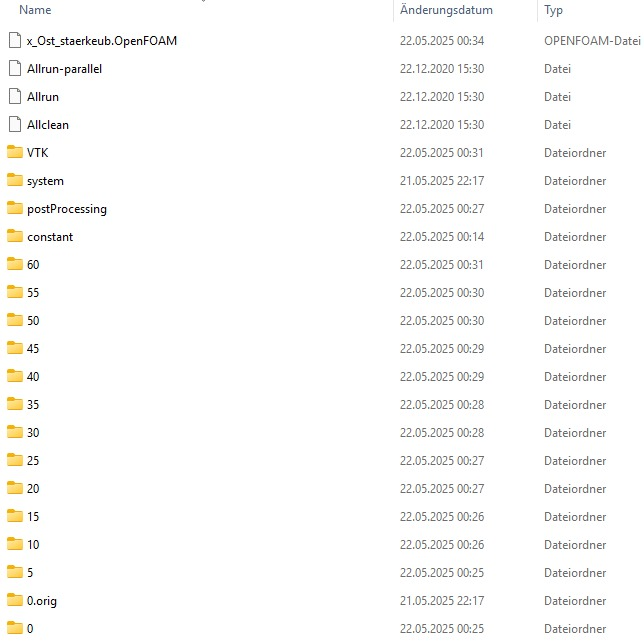
\includegraphics[width=0.55\textwidth]{papers/openfoam/Bilder/Ordnerstruktur_Simuliert.jpg}
    \caption{Ordnerstruktur nach der Simulation, 0,5...60 die Zeitpunkte, die in Paraview dargestellt werden können.}
    \label{fig:ordStrktSim}
\end{figure}

%Vorbereitung Kapitel --------------------------------------------------------------------------------------
\subsection{Vorbereitung \label{openfoam:section:Vorbereitung}}
Bevor mit der Simulation begonnen wird, müssen einige Entscheidungen getroffen werden.
\begin{itemize}
    \item Es muss entschieden werden, was überhaupt simuliert werden möchte und welche Gleichungen dafür infrage kommen.
    Zum Beispiel die Navier-Stokes-Gleichungen, Large-Eddy Simulation oder auch solche für Wärmeübertragung.
    \item Es muss die Geometrie der Umgebung definiert werden. 
    Gibt es Möglichkeiten Symmetrien auszunutzen, um den Rechenaufwand zu minimieren?
    \item Die Randbedingungen müssen festgelegt werden, wo strömt das Fluid in die Simulation ein, wo verlässt es sie.
    \item Wie verhalten sich die Wände, tragen sie zu Turbulenzen bei oder nicht?
    \item Sind die Wände genug weit vom Modell entfernt, dass ihr Einfluss auf das Ergebnis vernachlässigbar ist?
\end{itemize} 
Diese Überlegungen sind essenziell, um ein realistisches und stabiles Simulationsmodell aufzubauen.

%Mesh erstellen Kapitel ------------------------------------------------------------------------------------
\subsection{Mesh erstellen \label{openfoam:section:Mesh erstellen}}
Der grundlegende Schritt einer jeden Simulation ist, die reale, analoge Welt in eine diskrete Welt zu überführen.
Der Simulationsraum wird mit dem Programm \textbf{blockMesh}\footnote{In diesem Paper wir die Notation: \textbf{Fett für Programme}, \textit{kursiv für Parameter} und \texttt{Monospace für Ordner und Dokumente} verwendet.} 
erstellt.
Im Dokument \texttt{blockMeshDict} werden die Parameter definiert:

\begin{itemize}
    \item \textit{backgroundMesh}: Definiert wie gross der Simulationsraum ist und wie er in diskrete Zelle unterteilt werden soll. Später baut das Programm \textbf{snappyHexMesh} darauf auf.
    \item \textit{boundary}: Beschreibt die Ränder des Simulationsraum, weist jeder Fläche einen Namen und eine Bedingung (Inlet, Outlet, Wand) zu
\end{itemize}
Die Zellen im Simulationsraum bilden die Grundlage für die Simulation. 
Je mehr Zellen erstellt werden, desto genauer wird das Ergebnis der Simulation, da die Berechnungen kleinräumiger erfolgen.
Mit jeder Zelle steigt jedoch der Rechenaufwand.
Es muss ein Mittelweg gefunden werden, so viele Zellen wie nötig, so wenige wie möglich.

Als nächstes wird das 3D-Modell in den Simulationsraum eingebettet.
Mithilfe dem Programm \textbf{snappyHexMesh} wird das 3D-Modell in  Zellen unterteilt und eingefügt. 
Im Dokument \texttt{snappyHexMeshDict} werden die Parameter definiert:

\begin{itemize}
    \item \textit{geometry}: Definition des 3D-Modells, zum Beispiel in Form einer STL-Datei.
    \item \textit{castellatedMeshControls}: Erste Stufe des Meshing, steuert, wie die Quader am Anfang angenähert werden.
    \item \textit{snapControls}: Wie oft das Mesh verfeinert wird. 
    In einem ersten Durchlauf wird das 3D-Modell grob in Quader aufgeteilt (Abb. \ref{fig:snappygrobbild}),
    in den folgenden Schritten wird die Annäherung an die Vorgabe immer besser (Abb. \ref{fig:snappyfeinbild}).
    Üblich sind 20 bis 40 Durchläufe, ist jedoch auch ein Abwägen zwischen dem Nutzen und dem erhöhten Rechenaufwand.
    \item \textit{addLayersControls}: Im 3D-Mesh werden die Blöcke in der Nähe des Modells verkleinert, 
    damit können die interessanten Bereiche räumlich genauer simuliert werden.
\end{itemize}
Spitze Kanten und Ecken korrekt darzustellen sind für \textbf{snappyHexMesh} eine Herausforderung.
Das Programm \textbf{surfaceFeatureExtract} wird verwendet um diese Bereiche gesondert aus dem 3D-Modell zu extrahieren.
Es wird vor \textbf{snappyHexMesh} ausgeführt und hilft, die Zellen genauer an der Geometrie auszurichten.
Im Dokument \texttt{surfaceFeatureExtractDict} werden die Parameter definiert:

\begin{itemize}
    \item \textit{3D-Modell}: Verweis auf das 3D-Modell von wo die Features extrahiert werden sollen.
    \item \textit{includedAngle}: Winkel, ab welchem eine Kante als spitz gilt und extrahiert wird.
\end{itemize}

\begin{figure}
    \centering
    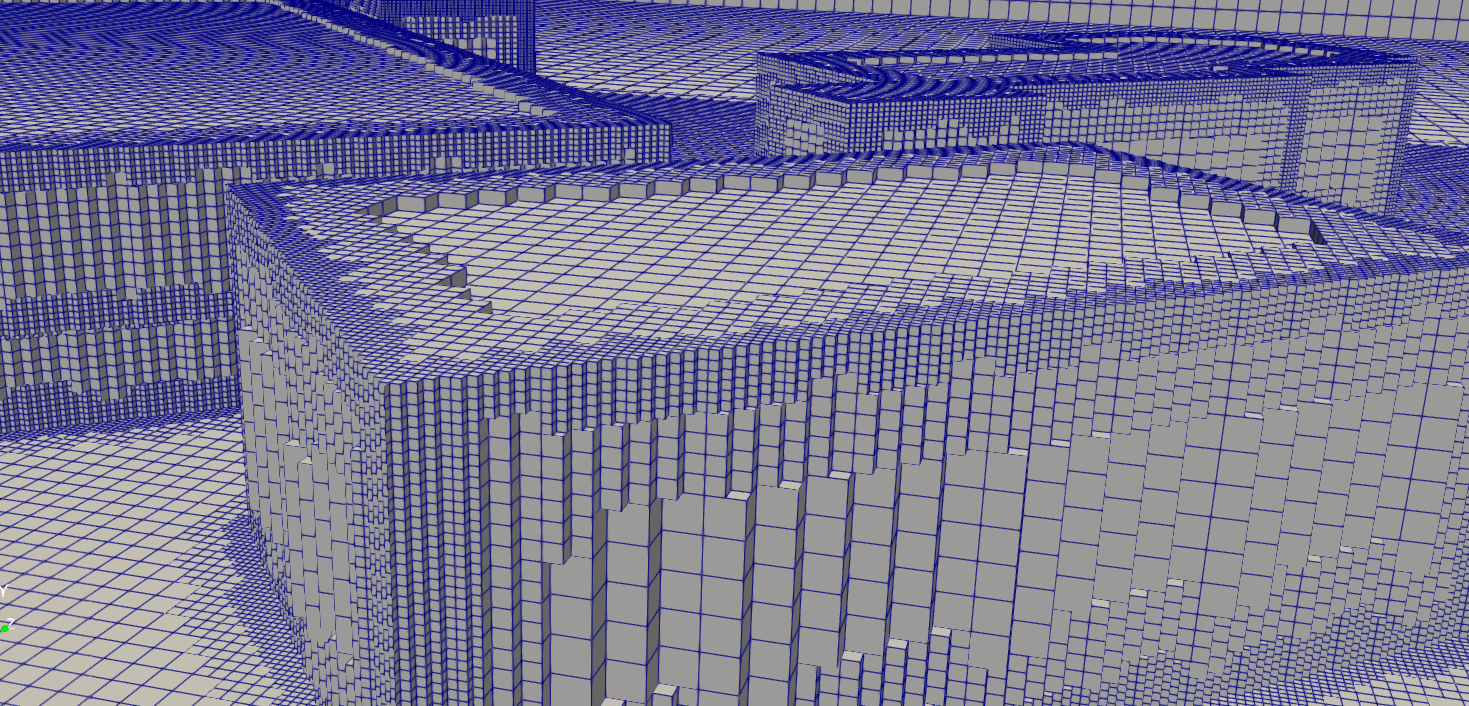
\includegraphics[width=0.55\textwidth]{papers/openfoam/Bilder/Snappy_grob.png}
    \caption{Mesh nach dem ersten Durchlauf von snappyHexMesh}
    \label{fig:snappygrobbild}
\end{figure}

\begin{figure}
    \centering
    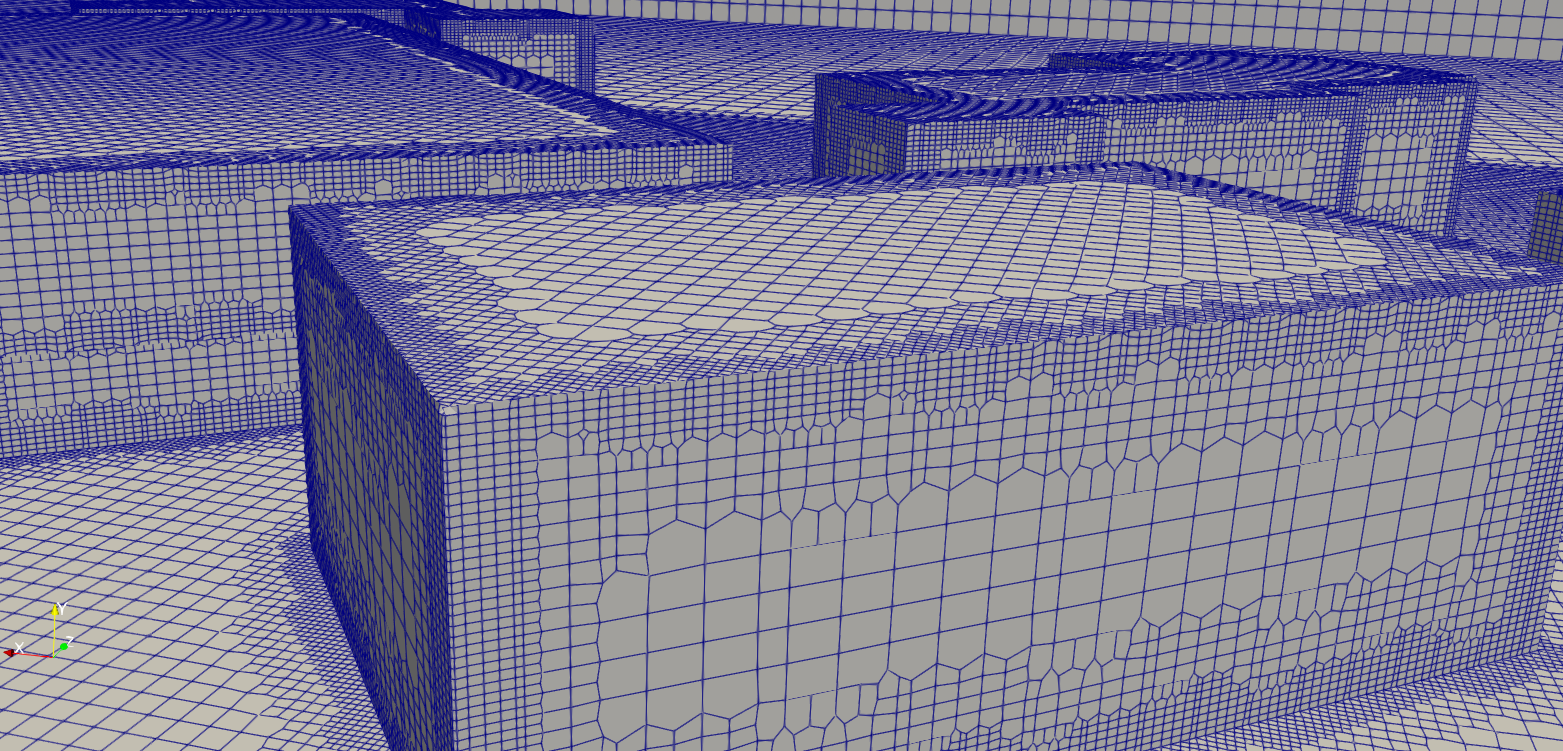
\includegraphics[width=0.55\textwidth]{papers/openfoam/Bilder/Snappy_fein.png}
    \caption{Mesh nach dem mehrfachen Durchlaufen von snappyHexMesh}
    \label{fig:snappyfeinbild}
\end{figure}

%Anfangsbedingungen Kapitel --------------------------------------------------------------------------------
\subsection{Anfangsbedingungen \label{openfoam:section:Anfangsbedingungen}}
Bei jeder Simulation muss beim ersten Zeitschritt ein Initialzustand definiert sein.
Alle Zellen müssen mit Startwerten versehen werden. 
Diese Werte werden im Ordner \texttt{0} hinterlegt:
\begin{itemize}
    \item \texttt{p}: Druck im Fluid [m²/s²]
    \item \texttt{U}: Geschwindigkeit und Richtung der Strömungsvektoren [m/s]\\
    \textit{Uinlet} $ (x, y, z) $ beschreibt die Richtung und Stärke der Strömung. 
    \item \texttt{epsilon}: Dissipationsrate der turbulenten kinetischen Energie [m²/s³]
    \item \texttt{k}: Turbulente kinematische Energie [m²/s²]
    \item \texttt{nut}: Turbulente kinematische Viskosität [m²/s]
\end{itemize}
\texttt{epsilon}, k und nut sind Teil von Turbulenzmodellen, in diesem Paper wird nicht weiter darauf eingegangen.

In allen Dokumenten für die unterschiedlichen Anfangsbedingungen gibt es die Variable \textit{dimensions}, sie bestimmt die Einheit des Wertes.
Wie angesprochen, sind die Dimensionen \texttt{[kg m s K mol A cd]}.
\texttt{[0 2 -3 0 0 0 0]} steht zum Beispiel für [m²/s³], der Einheit von epsilon.

%Parameter Kapitel ----------------------------------------------------------------------------------------
\subsection{Steuerparameter \label{openfoam:section:Steuerparameter}}
Für die Simulation müssen diverse Konstanten und Steuerparameter in den Dokumenten die in den Ordnern \texttt{system} und \texttt{constant} hinterlegt sind, definiert werden.

Im Ordner \texttt{constant} werden im Dokument \texttt{transportProperties} das \textit{transportModel} für die Viskosität und einen Wert, \textit{nu}, für die kinematische Viskosität gesetzt.
Für Fluide mit konstanter Viskosität wird das Modell Newtonian verwendet. Bei Luft zum Beispiel \textit{nu} = 1.82e -5, \textit{transportModel} = Newtonian

Ebenfalls im Ordner \texttt{constant} im Dokument \texttt{turbulenceProperties} wird der \textit{simulationType} festgelegt, dieser beschreibt wie OpenFOAM die Turbulenzen simuliert.
Zum Beispiel Reynolds-averaged Simulation (RAS), Large Eddy Simulation (LES) oder laminar.

Der Ordner \texttt{system} enthält das Dokument \texttt{controlDict}. Damit wird der zeitliche Ablauf der Simulation gesteuert.

\begin{itemize}
    \item \textit{application}: In unserem Fall, stationär und inkompressibel, 
    verwenden wir simpleFoam. Es gibt jedoch für jeden Anwendungsbereich eigene Solver.

    Eine unvollstänige Übersicht:
    \begin{itemize}
        \item icoFoam: zeitabhängig, inkompressibel, laminar
        \item buoyantSimpleFoam: stationär, inkompressibel, Wärmeübergang
        \item sonicFoam: zeitabhängig, kompressibel
    \end{itemize}
    \item \textit{startTime}: Startzeit der Simulation [s]
    \item \textit{endTime}: Endzeit der Simulation [s]
    \item \textit{deltaT}: Zeitschritt der Simulation [s]
    \item \textit{writeInterval}: Legt fest, welche Zeitordner erzeugt werden (Abb. \ref{fig:ordStrktSim}).
\end{itemize}

%fvSchemes TODO

%fvSolution TODO

%Simulation Kapitel ----------------------------------------------------------------------------------------
\subsection{Simulation \label{openfoam:section:Simulation}}
In der Simulation wird nun auf jede Zelle das in den Parametern definierte Gleichungssystem angewendet.
Die Berechnungen basieren auf den festgelegten Anfangs- und Randbedingungen sowie dem gewählten Solver.

Mit der folgenden Befehlsfolge kann eine einfache Simulation, stationär und inkompressibel, anhand eines Beispiel-Cases durchgeführt werden:

\begin{enumerate}
    \item \textbf{blockMesh}: Generiert Simulationsraum.
    \item \textbf{surfaceFeatureExtract}: Extrahiert scharfe Kanten und Ecken aus dem 3D-Modell.
    \item \textbf{snappyHexMesh}: Fügt das 3D-Modell in den Simulationsraum ein.
    \item \textbf{simpleFoam}: Simulation, bei einem anderen Solver durch den entsprechenden ersetzen.
    \item \textbf{foamToVTK}: (nicht nötig, wenn die Ergebnisse auf Linux mit \texttt{paraFoam} ausgewertet werden)\\
    Exportiert die Simulationsergebnisse in ein VTK-kompatibles Format, welches dann in \texttt{ParaView} angesehen werden kann.
    \item \textbf{paraFoam -touch}: (nicht nötig, wenn die Ergebnisse auf Linux mit \texttt{paraFoam} ausgewertet werden)\\
    Erstellt eine Projektdatei, die dann in \texttt{ParaView} geöffnet werden kann.
\end{enumerate}

Für das Ausführen der Befehle muss in der Kommandozeile in den \texttt{Case}-Ordner navigiert werden, in diesem Fall befindet sich der Ordner an der Position:\\
\texttt{/OpenFOAM/OpenFOAM-v2012/tutorials/incompressible/simpleFoam/}-\\
\texttt{Case\_Ordner}

Dort können dann die Befehle nacheinander eingegeben werden.
Erfahrungsgemäss kann \textbf{snappyHexMesh} und \textbf{simpleFoam}, je nach Einstellungen und Komplexität des 3D-Modells, 
lange dauern, mehrere Stunden sind möglich.
Grosse Simulationen können mehrere 100 GB an Speicherplatz benötigen.

Es wird empfohlen mit einfachen Modellen, Tutorials und kurzen Simulationszeiten anzufangen.

%Auswertung Kapitel ----------------------------------------------------------------------------------------
\subsection{Auswertung \label{openfoam:section:Auswertung}}
Nach der Simulation können die Ergebnisse ausgewertet werden. 
Wir verwenden \texttt{ParaView} für die Auswertung. 
Auf Linux-Systemen ist \texttt{paraFoam} verfügbar, dies wird hier jedoch nicht weiter verfolgt.
Die Ergebnisse können auch mit einem eigenen \texttt{Skript} ausgewertet und weiterverarbeitet werden.

In ParaView öffnet man das \texttt{Case\_Ordner.OpenFOAM} Dokument im \texttt{Case}-Ordner.
Abbildung \ref{fig:Beispiel_Paraview} zeigt die wichtigsten Bedienelemente.
Für ein aussagekräftiges Ergebnis sollten die ersten Zeitschritte ignoriert werden, die Simulation braucht eine gewisse Zeit, bis sie einen stationären Zustand eingenommen hat.

Mithilfe diverser Einstellmöglichkeiten für die Darstellung wird aus \ref{fig:Beispiel_Paraview} das Umschlagbild des Buches.
Abbildung \ref{fig:vorschWindWestBlocky} zeigt dasselbe Ergebnis, jedoch mit der Einstellung, dass die einzelnen Zellen des Mesh sichtbar sind.

\begin{figure}
    \centering
    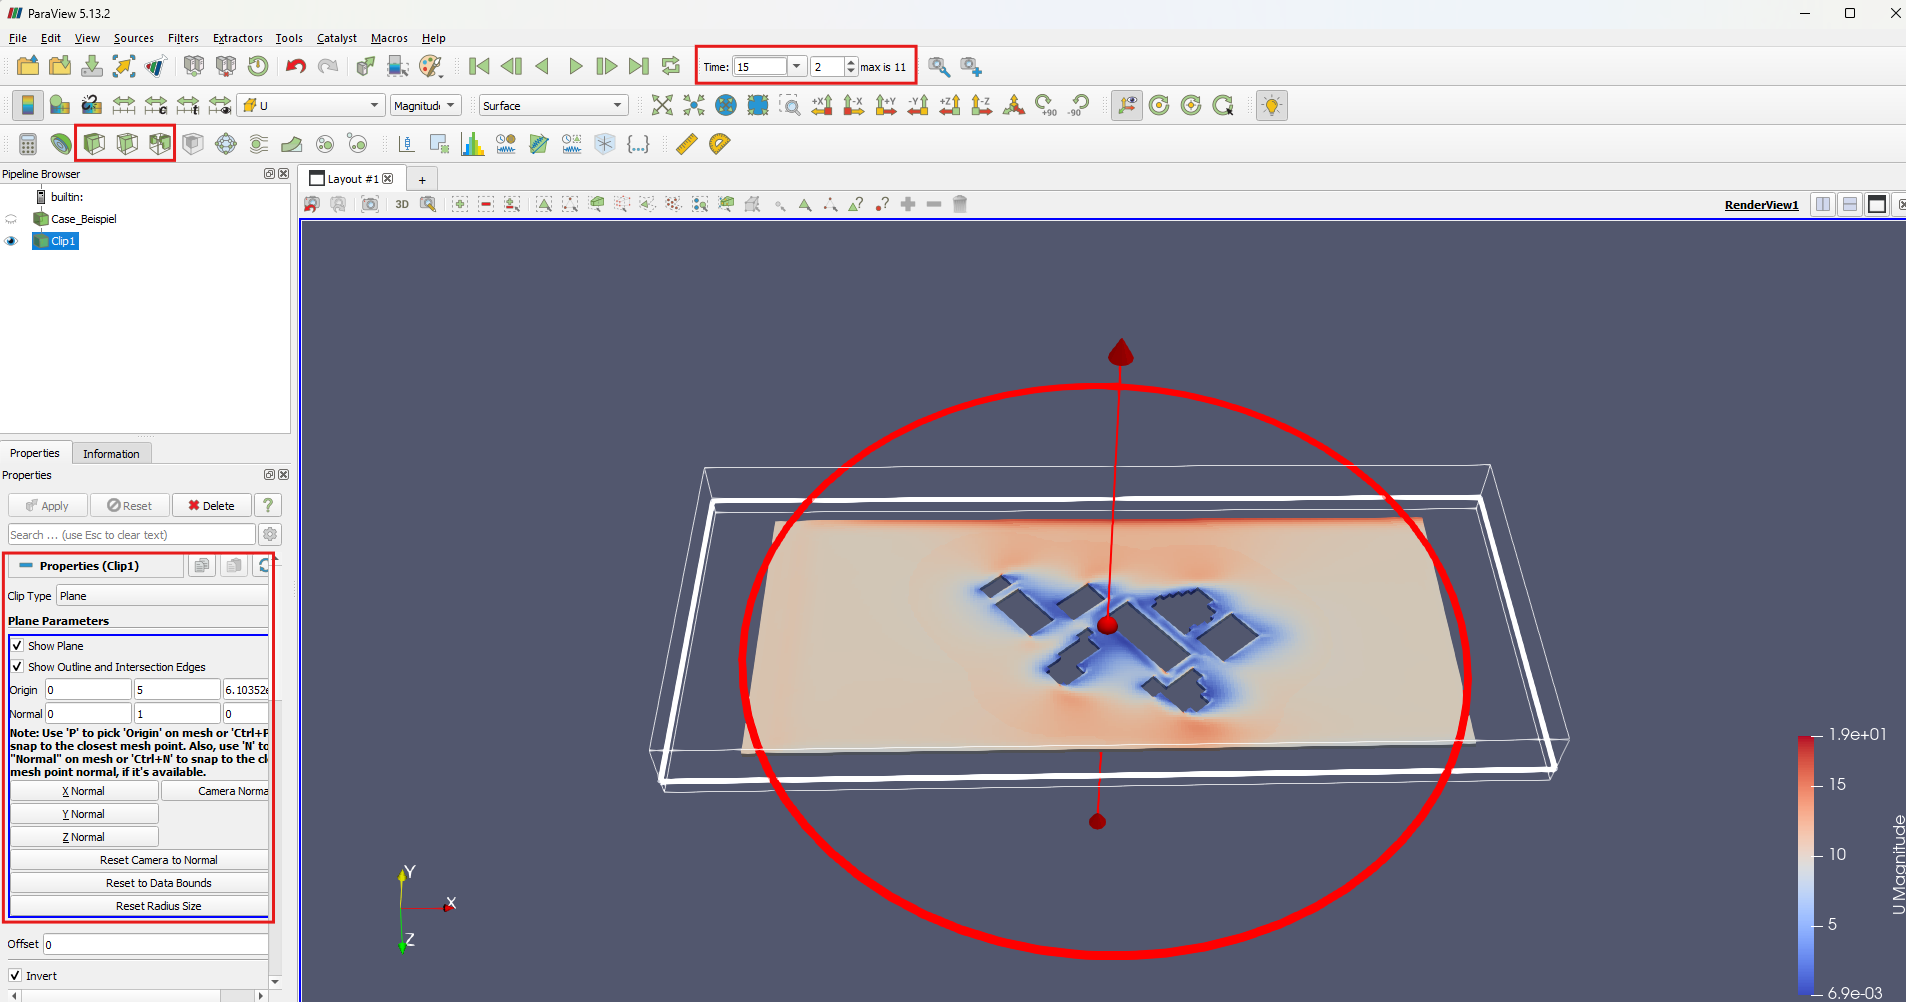
\includegraphics[width=1\textwidth]{papers/openfoam/Bilder/Beispiel_Paraview.png}
    \caption{Bedienung von \texttt{ParaView}\\ oben links: slice auswählen\\ oben mitte: Zeitschritte\\ unten links: Parameter}
    \label{fig:Beispiel_Paraview}
\end{figure}

\begin{figure}
    \centering
    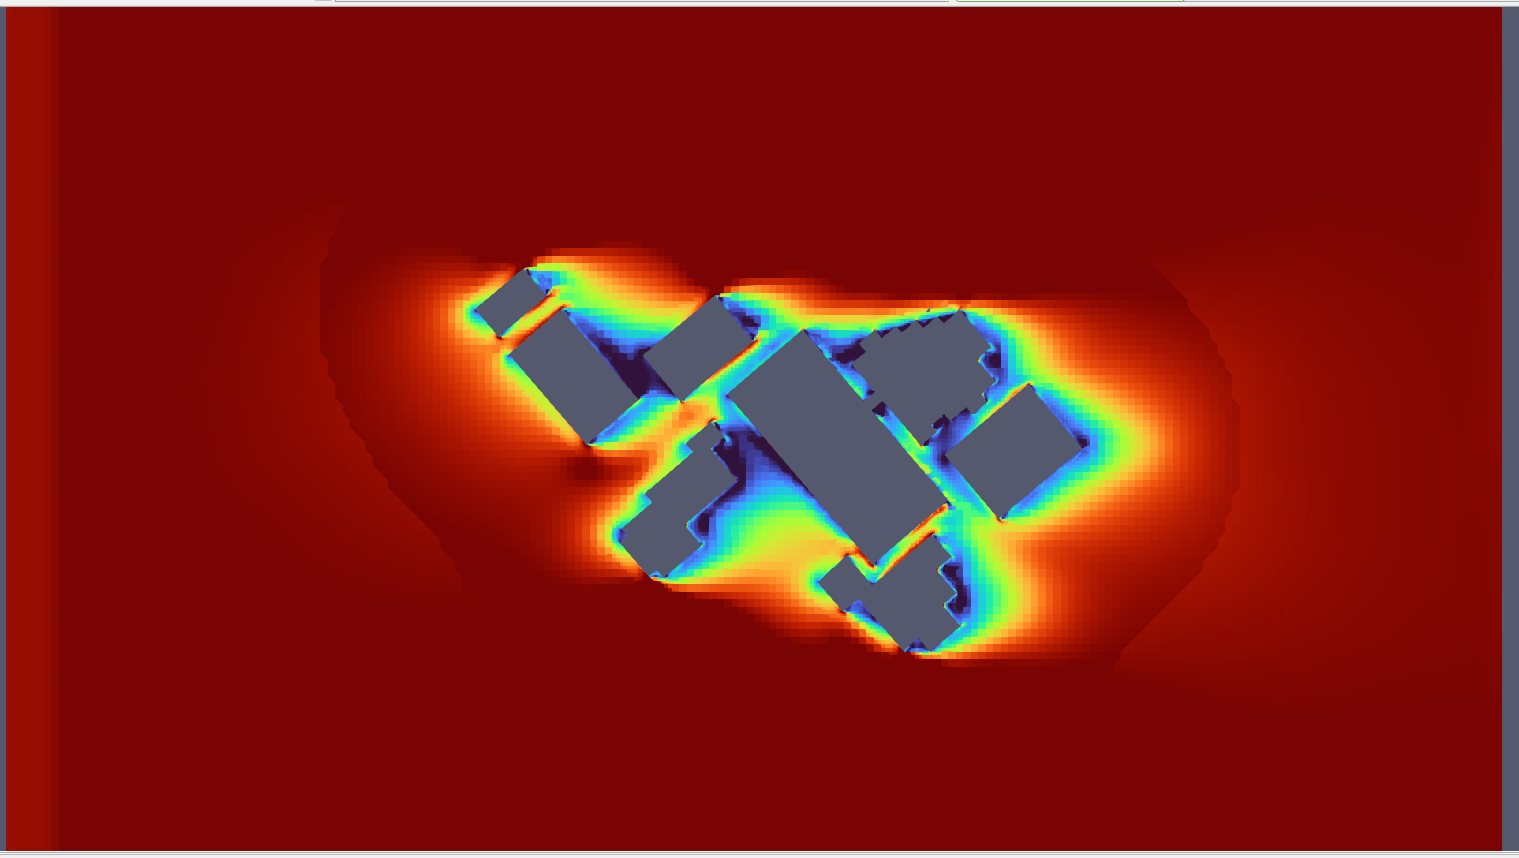
\includegraphics[width=1\textwidth]{papers/openfoam/Bilder/vorschlag_Wind_Westen_10m_blocky.png}
    \caption{Gleiches Bild wie auf dem Buchumschlag, jedoch mit den einzelnen Simulationszellen sichtbar.}
    \label{fig:vorschWindWestBlocky}
\end{figure}

Bei der Auswertung ist zu berücksichtigen, dass digitale Modelle die Realität nur näherungsweise abbilden. 
Daher stellt auch jede Simulation lediglich eine vereinfachte Repräsentation der realen Vorgänge dar und muss, bei Bedarf, mit physischen Experimenten validiert werden.
